\chapter{Metodología}

\section{Enfoque metodológico}
El desarrollo del proyecto se estructuró siguiendo el modelo de proceso CRISP-DM \cite{wirth2000}, cuyas seis fases se mapearon al trabajo realizado de la siguiente manera: la \textit{comprensión del negocio} corresponde al levantamiento del proceso de creación de materiales y a la cuantificación de su problemática; la \textit{comprensión de los datos}, al análisis exploratorio del maestro exportado desde SAP; la \textit{preparación de los datos}, a la construcción del pipeline de integración y del conjunto de modelado; el \textit{modelado}, a la evaluación comparativa de algoritmos de clasificación; la \textit{evaluación}, a la medición del desempeño sobre datos retenidos y sobre la operación real; y el \textit{despliegue}, a la puesta en producción de la plataforma y a su uso por parte del equipo de gestores.

La ejecución no fue lineal. Los hallazgos del análisis exploratorio —en particular la distribución fuertemente asimétrica de materiales entre categorías— obligaron a volver sobre la definición del conjunto de modelado, y los resultados de la primera competencia de algoritmos motivaron una segunda ronda de evaluación con familias adicionales.

\section{Materiales}

\subsection{Fuentes de información}
La fuente primaria del proyecto es el maestro de materiales del módulo MM de SAP correspondiente a la unidad de negocio. Al no existir integración directa con el ERP, la extracción se realizó mediante exportación manual a archivos de hoja de cálculo, organizados en trece archivos según el tipo de material. Cada registro aporta el código de material, su texto breve —la descripción normalizada de hasta cuarenta caracteres—, la denominación estándar que actúa como categoría, y la unidad de medida base.

A esta fuente se sumaron dos catálogos de referencia. El primero es el maestro de clases o denominaciones de la corporación, con 1,538 entradas, que además del código y el nombre de cada clase aporta el grupo de artículos, el sector, el tipo de material asociado y su correspondencia con el clasificador UNSPSC. El segundo es la tabla del propio clasificador UNSPSC de Naciones Unidas \cite{undp2023}, que permite anclar la taxonomía interna a un referente externo estandarizado.

Todas las fuentes son de naturaleza estructurada y de acceso directo dentro de la unidad de negocio. El corte del maestro empleado para el desarrollo y el entrenamiento corresponde a una fecha específica de extracción, lo que implica que el catálogo con el que opera la plataforma es una fotografía y no un reflejo en tiempo real del ERP.

\subsection{Recursos tecnológicos}
La plataforma se construyó sobre PostgreSQL 16 con la extensión \texttt{pg\_trgm} habilitada, un API desarrollado en Python con FastAPI, un entorno de Jupyter Lab para la experimentación analítica y un frontend de página única servido por Nginx, todo orquestado mediante contenedores con Docker Compose. El modelado se realizó con las bibliotecas estándar del ecosistema científico de Python. La normalización de descripciones se apoya en un modelo de lenguaje de gran escala consumido por interfaz de programación.

Con la única excepción del servicio de modelo de lenguaje, que opera bajo un esquema de pago por uso, la totalidad de la infraestructura se compone de software de código abierto.

\section{Integración de la información}

\subsection{Arquitectura implementada}
El repositorio de datos se implementó siguiendo la arquitectura medallón descrita en el marco teórico, con cuatro esquemas de responsabilidad diferenciada. El esquema \texttt{bronze} concentra la trazabilidad del sistema: registros de ingesta, de predicciones, de decisiones sobre duplicados, de interacciones con el modelo de lenguaje y de errores de aplicación. El esquema \texttt{silver} contiene los datos operacionales y de referencia ya normalizados: el maestro de materiales, los catálogos de clases, tipos de material, unidades de medida y UNSPSC, además de las conversaciones y las solicitudes de alta. El esquema \texttt{gold} expone vistas agregadas para el consumo del tablero de indicadores. Un cuarto esquema alberga la administración de usuarios de la plataforma.

La elección de un motor relacional en lugar de una plataforma distribuida responde al volumen de datos involucrado: un catálogo de decenas de miles de registros no justifica la complejidad operativa de un entorno de procesamiento distribuido, y permite además resolver la detección de duplicados dentro del mismo motor, sin necesidad de un servicio de búsqueda externo.

\subsection{Proceso de ingesta}
La carga de los archivos se implementó como un conjunto de servicios del API que reciben el archivo, lo interpretan y lo depositan en las tablas correspondientes. El proceso aplica un mapeo explícito entre los encabezados originales de la exportación de SAP y los campos del modelo de datos, resuelve los casos en que la exportación repite un mismo nombre de columna, y extrae los códigos de aquellos campos que llegan como valores compuestos de código y descripción separados por un guion.

Durante la carga se resuelven las llaves foráneas contra los catálogos de referencia: cada material se vincula con su clase y su unidad de medida, y cada clase con su tipo de material y su código UNSPSC. Toda ejecución queda registrada con el nombre del archivo, el número de filas procesadas, el estado resultante, el mensaje de error en caso de fallo y el tiempo transcurrido, lo que permite auditar el origen de cualquier registro del maestro.

Sobre la columna de texto breve del maestro se construyó un índice invertido de trigramas, que es el que sostiene el desempeño de las consultas de similitud.

\section{Preparación de los datos}

\subsection{Preprocesamiento de texto}
Para el modelado se definió una función de normalización que convierte el texto a mayúsculas, descompone y elimina los signos diacríticos, sustituye por espacios los separadores propios de la convención de nomenclatura, descarta los caracteres que no son alfanuméricos ni punto o guion, y colapsa los espacios redundantes. Esta transformación conserva las dimensiones, fracciones y designaciones técnicas, que son precisamente los elementos discriminantes en una descripción de material.

Una consideración crítica de diseño es que esta función es la misma en el entrenamiento y en la inferencia. Un modelo entrenado sobre texto preprocesado de una forma y consultado con texto preprocesado de otra degrada su desempeño de manera silenciosa, sin producir ningún error visible.

\subsection{Criterios de construcción del conjunto de modelado}
Sobre el maestro consolidado se aplicaron dos criterios de exclusión. El primero descarta los materiales que no tenían categoría asignada en la fuente, por no poder emplearse ni para entrenar ni para evaluar. El segundo descarta las clases representadas por menos de tres ejemplos, por resultar insuficientes para permitir simultáneamente el entrenamiento y la evaluación de una misma categoría.

El conjunto resultante se particionó en entrenamiento y prueba en proporción aproximada de 80 y 20 por ciento. La partición se estratificó por clase, dado el desbalance observado en el análisis exploratorio.

\section{Métodos analíticos}

\subsection{Normalización de descripciones mediante modelo de lenguaje}
El módulo de normalización se resolvió mediante un modelo de lenguaje de gran escala consumido a través de su interfaz de programación, en lugar de un motor de reglas y diccionarios de abreviatura. Esta decisión se sustenta en la evidencia de que los modelos fundacionales alcanzan desempeño competitivo en tareas de limpieza y estandarización de datos sin entrenamiento específico \cite{narayan2022}, y en la consideración práctica de que un diccionario de abreviaturas exigiría mantenimiento manual permanente conforme aparecen materiales de familias nuevas.

El modelo se configuró con una temperatura baja, para privilegiar la consistencia sobre la variedad en la redacción, y con respuesta forzada en formato JSON, de manera que su salida pueda consumirse de forma programática sin análisis sintáctico frágil. La instrucción de sistema codifica cuatro elementos: las reglas de la convención corporativa de nomenclatura —límite de cuarenta caracteres, estructura de tipo y subtipo seguida de atributos, uso de mayúsculas, ausencia de tildes y abreviaturas estándar—; un conjunto de ejemplos tomados del propio maestro, que operan como demostraciones en contexto \cite{brown2020}; el catálogo de tipos de material vigente, inyectado dinámicamente desde la base de datos; y un protocolo de comportamiento ante información incompleta.

Este último elemento merece detalle. El modelo tiene instruido no inventar especificaciones ausentes: cuando la descripción que recibe es insuficiente, en lugar de completar con valores plausibles debe devolver una lista estructurada de los campos que faltan. Se definieron además reglas de dominio explícitas, como la obligatoriedad del material de fabricación para materiales físicos y la restricción de solicitar marca y modelo únicamente cuando se trata de repuestos o componentes en los que la marca es indispensable para la identificación. El diseño busca que el modelo falle por omisión y no por invención, que es el modo de falla aceptable en un proceso de gobierno de datos.

Cada interacción con el modelo se registra íntegramente: la instrucción enviada, la respuesta cruda, la respuesta interpretada, la acción resultante, el consumo de unidades de texto y el tiempo transcurrido.

\subsection{Detección de duplicados}
La detección de duplicados se implementó como una consulta de similitud difusa ejecutada directamente sobre el maestro normalizado, aprovechando la extensión \texttt{pg\_trgm} de PostgreSQL y el índice invertido de trigramas construido durante la ingesta \cite{gravano2001}. La consulta calcula el coeficiente de similitud entre la descripción propuesta y cada descripción del catálogo, retiene aquellas que superan un umbral configurable y devuelve las diez coincidencias de mayor puntaje ordenadas de forma descendente.

El umbral de alerta se estableció en un valor deliberadamente permisivo, bajo el criterio de que en una herramienta de asistencia el costo de un falso positivo —que el gestor descarte una sugerencia irrelevante— es sustancialmente menor que el de un falso negativo, que se materializa en un duplicado creado y en el costo recurrente de arrastrarlo en el catálogo.

Cuando la consulta arroja coincidencias, estas no se presentan al gestor como una lista cruda: se devuelven al modelo de lenguaje, que las expone en el contexto de la conversación señalando las diferencias relevantes entre el material propuesto y los candidatos encontrados. La decisión del gestor —aceptar uno de los materiales existentes o sostener que el suyo es distinto— se registra de forma explícita, junto con el conjunto de candidatos que se le presentó y el tiempo que tomó decidir.

\subsection{Diseño de la evaluación de algoritmos de clasificación}
La selección del algoritmo se resolvió mediante una competencia entre familias, evaluadas todas sobre la misma partición de datos y con las mismas métricas. En una primera ronda se evaluaron cuatro configuraciones que combinan dos representaciones vectoriales —TF-IDF de palabras y TF-IDF de n-gramas de carácter— con tres algoritmos: regresión logística, máquina de vectores de soporte lineal y bosque aleatorio. En una segunda ronda se incorporaron tres familias adicionales: potenciación de gradiente sobre árboles, un clasificador de subpalabras y un transformador multilingüe preentrenado sometido a ajuste fino.

Se privilegió la representación por n-gramas de carácter sobre la de palabras completas por la densidad de abreviaturas, fracciones y designaciones alfanuméricas del catálogo, y se configuró con ventanas de dos a cinco caracteres delimitadas por palabra, ponderación logarítmica de la frecuencia y un vocabulario acotado a cincuenta mil rasgos.

La máquina de vectores de soporte se envolvió en un procedimiento de calibración con validación cruzada de tres particiones. Esta decisión no fue accesoria: sin estimaciones de probabilidad la plataforma no puede aplicar un umbral de confianza, y sin umbral no puede distinguir las sugerencias que presenta como resueltas de las que somete a revisión explícita del gestor.

La comparación se realizó sobre exactitud global, ambos promedios de F1, exactitud sobre las tres primeras sugerencias y tiempo de entrenamiento; este último se incorporó como criterio porque un modelo que exige horas de cómputo para reentrenarse resulta inviable de mantener en la operación. La configuración ganadora se reentrenó sobre la totalidad del conjunto para su despliegue, por lo que las métricas que se reportan corresponden a la partición retenida y no al artefacto en producción.

Para determinar el punto de operación del sistema se caracterizó adicionalmente el compromiso entre exactitud y cobertura a distintos umbrales de confianza, siguiendo el planteamiento de clasificación con opción de rechazo \cite{chow1970}.

\section{Arquitectura tecnológica e implementación}

\subsection{Componentes y despliegue}
La plataforma se despliega mediante contenedores orquestados con Docker Compose, en cuatro servicios: el motor de base de datos con la extensión de similitud habilitada; el API, que concentra la lógica de negocio, la autenticación y la inferencia del modelo de clasificación; el entorno de experimentación analítica; y el frontend, que además actúa como proxy inverso hacia los demás servicios.

Una decisión de arquitectura relevante fue integrar la inferencia del modelo dentro del propio API en lugar de exponerla como un servicio independiente. El artefacto entrenado se carga en memoria una sola vez al arrancar el proceso y se reutiliza en cada predicción, lo que elimina la latencia de red entre servicios y la complejidad operativa de un componente adicional, a cambio de acoplar el ciclo de vida del modelo al del API.

\subsection{Ciclo de vida de una solicitud}
Una solicitud de alta atraviesa una secuencia definida de estados. Se crea en estado pendiente en el momento en que el modelo de lenguaje produce una propuesta de descripción normalizada. A partir de ahí puede resolverse de tres maneras: confirmarse, cuando el gestor valida la descripción y la categoría; descartarse, cuando la solicitud no procede; o cerrarse como coincidencia con un material existente, cuando la revisión de duplicados determina que el material ya está en el catálogo. Las solicitudes confirmadas transitan finalmente al estado exportado una vez incluidas en el archivo de entrega.

Este último estado materializa el punto de contacto con SAP. Las solicitudes validadas se consolidan en un archivo de hoja de cálculo que incorpora la descripción normalizada, la descripción extendida, el tipo de material, la clase asignada y las marcas de tiempo del proceso; ese archivo es el insumo con el que el material se registra en el ERP. La plataforma no escribe en SAP en ningún momento.

\section{Instrumentación y medición}
La medición del efecto de la herramienta no se resolvió de forma retrospectiva sino instrumentando el sistema desde su diseño, de modo que cada solicitud deje registro de su propio recorrido.

Cada solicitud almacena marcas de tiempo diferenciadas para su creación, la finalización de la normalización, la finalización de la búsqueda de duplicados, la decisión del gestor sobre los duplicados presentados, la finalización de la predicción de categoría, y su confirmación, descarte o exportación. Junto a ellas se registran las duraciones de cada etapa automática y su suma. Esta granularidad permite separar dos magnitudes que de otro modo quedarían confundidas: el tiempo que consume la máquina y el tiempo que consume la deliberación del gestor.

Se registra asimismo la calidad de la sugerencia. Cuando la clase que el gestor selecciona difiere de la que el modelo propuso, la solicitud queda marcada como corregida, lo que permite estimar la exactitud del modelo en operación real sobre datos que no formaron parte de su evaluación. Se registra también si la sugerencia superó el umbral de confianza y la confianza efectivamente obtenida.

Sobre esta base se construyó la capa de indicadores del esquema \texttt{gold}, materializada como vistas que agregan por semana los tiempos de procesamiento, la calidad de las predicciones, las decisiones sobre duplicados, el desglose por etapa del proceso, la actividad por usuario y el ahorro estimado. El cálculo del ahorro se parametriza mediante una tabla de configuración que almacena el tiempo de referencia del proceso manual y el costo por hora del gestor, de modo que el indicador pueda recalcularse ante un cambio de supuestos sin modificar la definición de la vista.

Todas las vistas de indicadores excluyen sistemáticamente la actividad de las cuentas administrativas. Esta exclusión es deliberada: el tráfico generado durante el desarrollo, las pruebas y las demostraciones contaminaría las mediciones de tiempo y de calidad si se agregara junto al uso productivo del equipo de gestores.

\section{Protocolo de validación en producción}
La validación de la herramienta se realizó mediante su uso efectivo por parte del equipo de gestores sobre solicitudes reales de la operación, durante el período comprendido entre el 18 de junio y el 21 de julio de 2026. La medición del efecto se construye por comparación contra una línea base del proceso manual levantada con anterioridad a la implementación, entre el 15 de febrero y el 17 de junio de 2026.

% ============================================================================
% PENDIENTE — completar con información que no está en el repositorio:
%
% 1. LÍNEA BASE. Cómo se midieron las 3.3 h por gestión, las 4.4 solicitudes
%    diarias y los 5–10 min de búsqueda manual: ¿registros de SAP, cronometraje,
%    entrevista con los gestores? Es el dato del que depende todo el ROI.
%
% 2. AUDITORÍA RETROACTIVA. Método con el que se obtuvieron los 456 duplicados
%    exactos, los 246 materiales mal categorizados, los 94 repuestos bajo
%    "suministros" y el 94 % de similitud parcial. Declarar el umbral usado
%    (el sistema opera con 0.45) y si el 94 % se midió a ese mismo valor.
%
% 3. CAPACITACIÓN. Número de gestores que usaron la herramienta, y si hubo
%    sesión inicial y sesión de seguimiento como se comprometió en Objetivos.
%
% 4. ENCUESTA. Si se aplicó, a quiénes, cuántos respondieron y con qué
%    instrumento. Si no se aplicó, hay que ajustar el objetivo correspondiente.
% ============================================================================


\chapter{Resultados}

\section{Caracterización del maestro de materiales}
La consolidación de los trece archivos de exportación produjo un total de 45,397 registros. La Figura \ref{fig:fuentes} muestra la composición del maestro según el archivo de origen: la distribución es marcadamente desigual, con dos tipos de material —repuestos industriales y suministros— que concentran por sí solos más del sesenta por ciento de los registros, mientras que varios tipos aportan menos de cien materiales cada uno.

\begin{figure}[!htb]
\centering
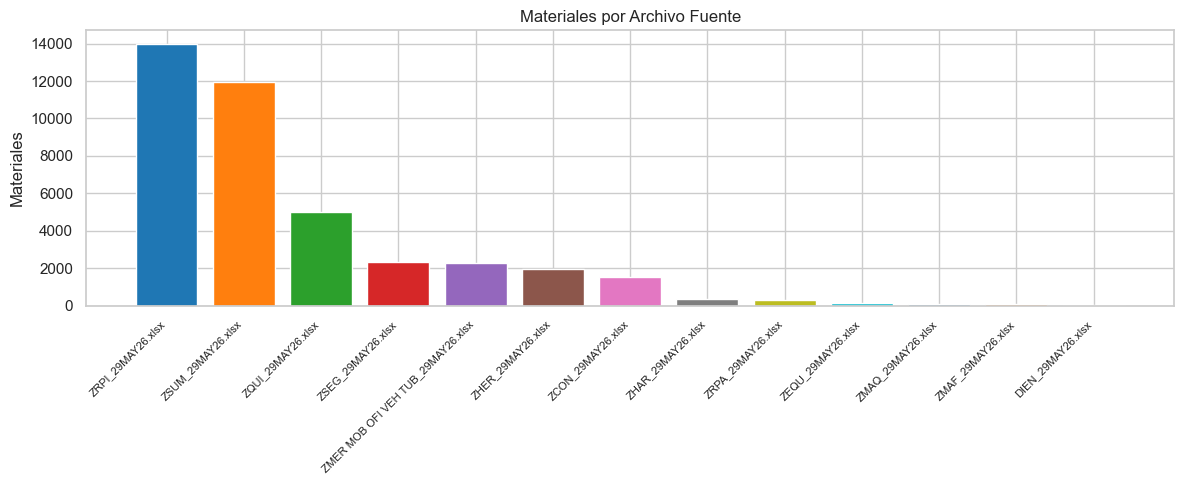
\includegraphics[width=\textwidth]{figuras/modelos/nb02_cell14.png}
\caption{Cantidad de materiales aportados por cada archivo de exportación del maestro}
\label{fig:fuentes}
\end{figure}

Del total de registros cargados, 40,029 contaban con una clase asignada en la fuente y 5,368 carecían de ella. Entre los materiales clasificados se identificaron 1,529 clases distintas, con una mediana de nueve materiales por clase y una clase máxima que concentra 655 registros. El Cuadro \ref{cuadro:distclases} detalla la distribución y la Figura \ref{fig:top20} presenta las veinte clases de mayor volumen.

\begin{table}[!htb]
\centering
\caption{Distribución de las clases del maestro según su cantidad de materiales}
\label{cuadro:distclases}
\begin{tabular}{lrr}
\toprule
\textbf{Materiales por clase} & \textbf{Clases} & \textbf{Participación} \\
\midrule
1 material          & 132   & 8.6\,\% \\
2 a 10 materiales   & 697   & 45.6\,\% \\
11 a 50 materiales  & 517   & 33.8\,\% \\
51 a 100 materiales & 103   & 6.7\,\% \\
Más de 100          & 80    & 5.2\,\% \\
\midrule
\textbf{Total}      & \textbf{1,529} & \textbf{100.0\,\%} \\
\bottomrule
\end{tabular}
\end{table}

Más de la mitad de las clases cuenta con diez materiales o menos, y 132 están representadas por un único registro.

\begin{figure}[!htb]
\centering
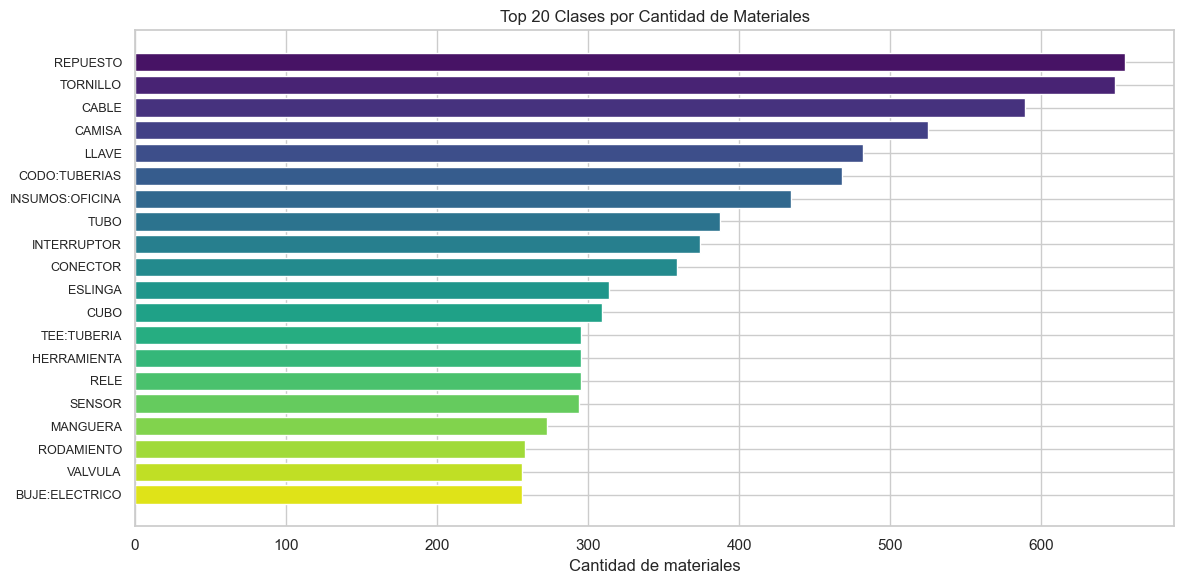
\includegraphics[width=\textwidth]{figuras/modelos/nb02_cell12.png}
\caption{Veinte clases con mayor cantidad de materiales en el maestro}
\label{fig:top20}
\end{figure}

En cuanto a la estructura del texto, las descripciones tienen una longitud media de 32.3 caracteres sobre un máximo posible de cuarenta, con una mediana de 34. La Figura \ref{fig:textostats} muestra que la distribución de longitudes se acumula abruptamente contra el límite de cuarenta caracteres. Cada descripción contiene en promedio 4.9 tokens y 2.3 separadores.

\begin{figure}[!htb]
\centering
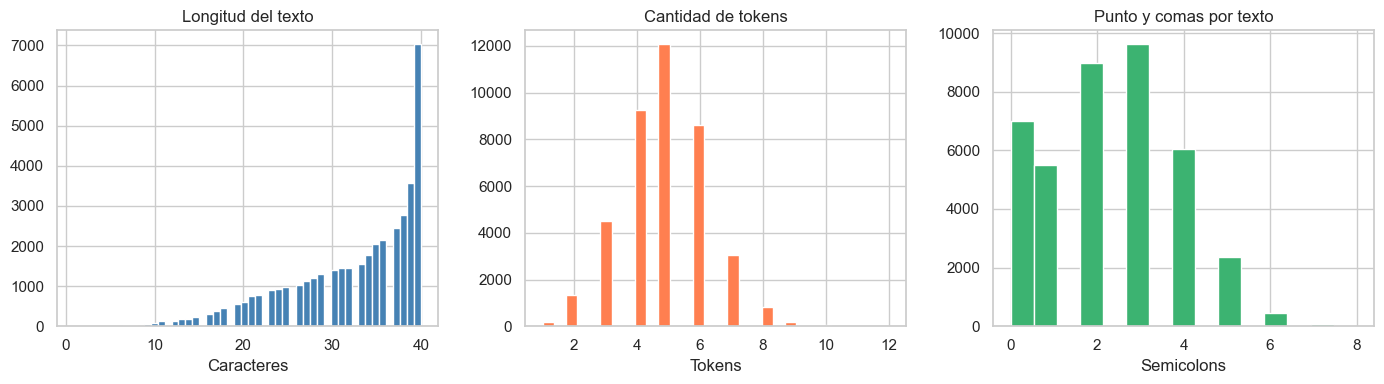
\includegraphics[width=\textwidth]{figuras/modelos/nb02_cell15.png}
\caption{Distribución de la longitud, cantidad de tokens y número de separadores de las descripciones del maestro}
\label{fig:textostats}
\end{figure}

\section{Conjunto de modelado resultante}
La aplicación de los criterios de exclusión definidos en la metodología produjo el conjunto que resume el Cuadro \ref{cuadro:embudo}. El descarte de los materiales sin categoría en la fuente eliminó 5,368 registros, y el de las clases con menos de tres ejemplos, 458 adicionales, para un conjunto final de 39,571 materiales distribuidos en 1,234 clases.

\begin{table}[!htb]
\centering
\caption{Construcción del conjunto de modelado a partir del maestro exportado}
\label{cuadro:embudo}
\small
\begin{tabular}{lrrl}
\toprule
\textbf{Etapa} & \textbf{Materiales} & \textbf{Clases} & \textbf{Criterio aplicado} \\
\midrule
Maestro exportado        & 45,397 & ---   & Trece archivos por tipo de material \\
Con clase asignada       & 40,029 & 1,529 & Se descartan 5,368 sin categoría en la fuente \\
Conjunto de modelado     & 39,571 & 1,234 & Se descartan clases con menos de tres ejemplos \\
\midrule
\quad Entrenamiento      & 31,656 & 1,234 & Partición estratificada, 80\,\% \\
\quad Prueba             & 7,915  & 1,234 & Partición estratificada, 20\,\% \\
\bottomrule
\end{tabular}
\end{table}

\section{Desempeño comparado de los algoritmos}
El Cuadro \ref{cuadro:competencia} presenta los resultados de las siete configuraciones evaluadas sobre la partición de prueba, y la Figura \ref{fig:compmodelos} contrasta gráficamente las métricas de la primera ronda.

\begin{table}[!htb]
\centering
\caption{Resultados de la competencia de algoritmos sobre la partición de prueba de 7,915 materiales y 1,234 clases}
\label{cuadro:competencia}
\small
\begin{tabular}{lrrrrr}
\toprule
\textbf{Configuración} & \textbf{Exactitud} & \textbf{F1 macro} & \textbf{F1 pond.} & \textbf{Top-3} & \textbf{Tiempo (s)} \\
\midrule
LinearSVC + TF-IDF carácter   & \textbf{0.8491} & \textbf{0.7523} & \textbf{0.8380} & \textbf{0.9404} & 62.9 \\
Random Forest + TF-IDF palabra & 0.8334 & 0.7360 & 0.8254 & 0.9263 & 46.7 \\
Reg. logística + TF-IDF carácter & 0.8293 & 0.6713 & 0.8126 & 0.9359 & 1,071.2 \\
Reg. logística + TF-IDF palabra  & 0.8291 & 0.6949 & 0.8178 & 0.9275 & 29.1 \\
XGBoost + TF-IDF carácter      & 0.8145 & 0.6821 & 0.8063 & 0.9200 & 11,025.2 \\
fastText                       & 0.8077 & 0.6897 & 0.8001 & 0.9075 & 43.0 \\
Transformer (MiniLM)           & 0.0395 & 0.0003 & 0.0050 & 0.0714 & 1,460.0 \\
\bottomrule
\end{tabular}
\end{table}

\begin{figure}[!htb]
\centering
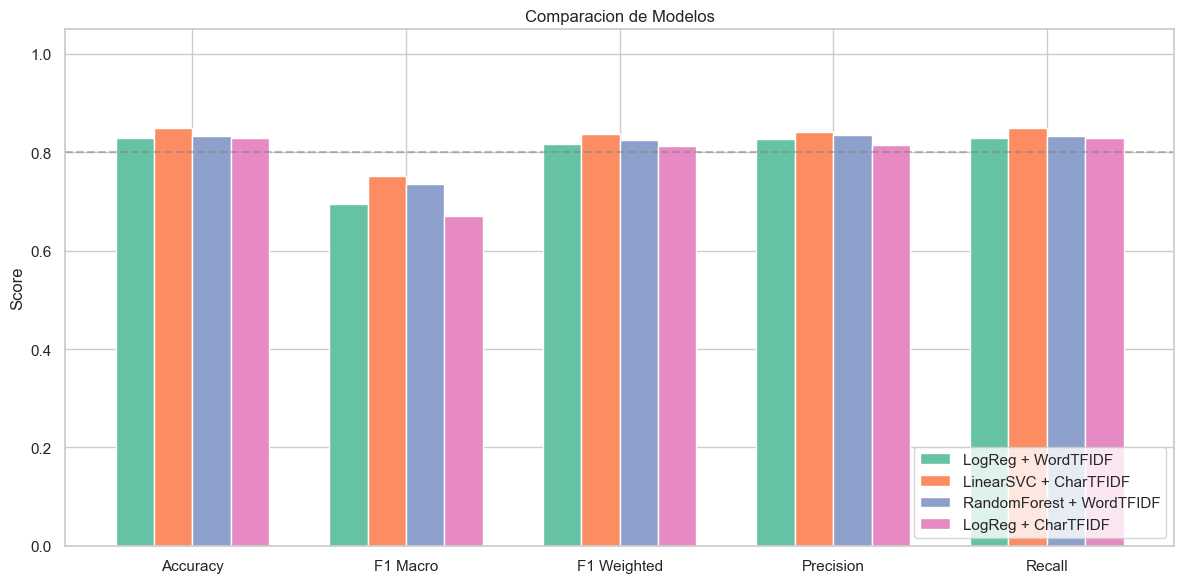
\includegraphics[width=\textwidth]{figuras/modelos/nb02_cell29.png}
\caption{Comparación de métricas entre las configuraciones evaluadas en la primera ronda}
\label{fig:compmodelos}
\end{figure}

La configuración de máquina de vectores de soporte lineal sobre TF-IDF de carácter obtuvo el mejor resultado en las cuatro métricas de desempeño, con una exactitud de 0.8491 y una exactitud sobre las tres primeras sugerencias de 0.9404, y fue la seleccionada para el despliegue.

\section{Desempeño del modelo seleccionado}
La Figura \ref{fig:matrizconf} presenta la matriz de confusión del modelo seleccionado sobre las veinte clases de mayor volumen. La diagonal concentra la mayor parte de los casos; las clases con vocabulario propio y estable —tornillo, camisa, codo de tubería, manguera— se resuelven casi sin error, mientras que las categorías de naturaleza genérica, como \textit{repuesto} o \textit{herramienta}, presentan las tasas de acierto más bajas del conjunto.

\begin{figure}[!htb]
\centering
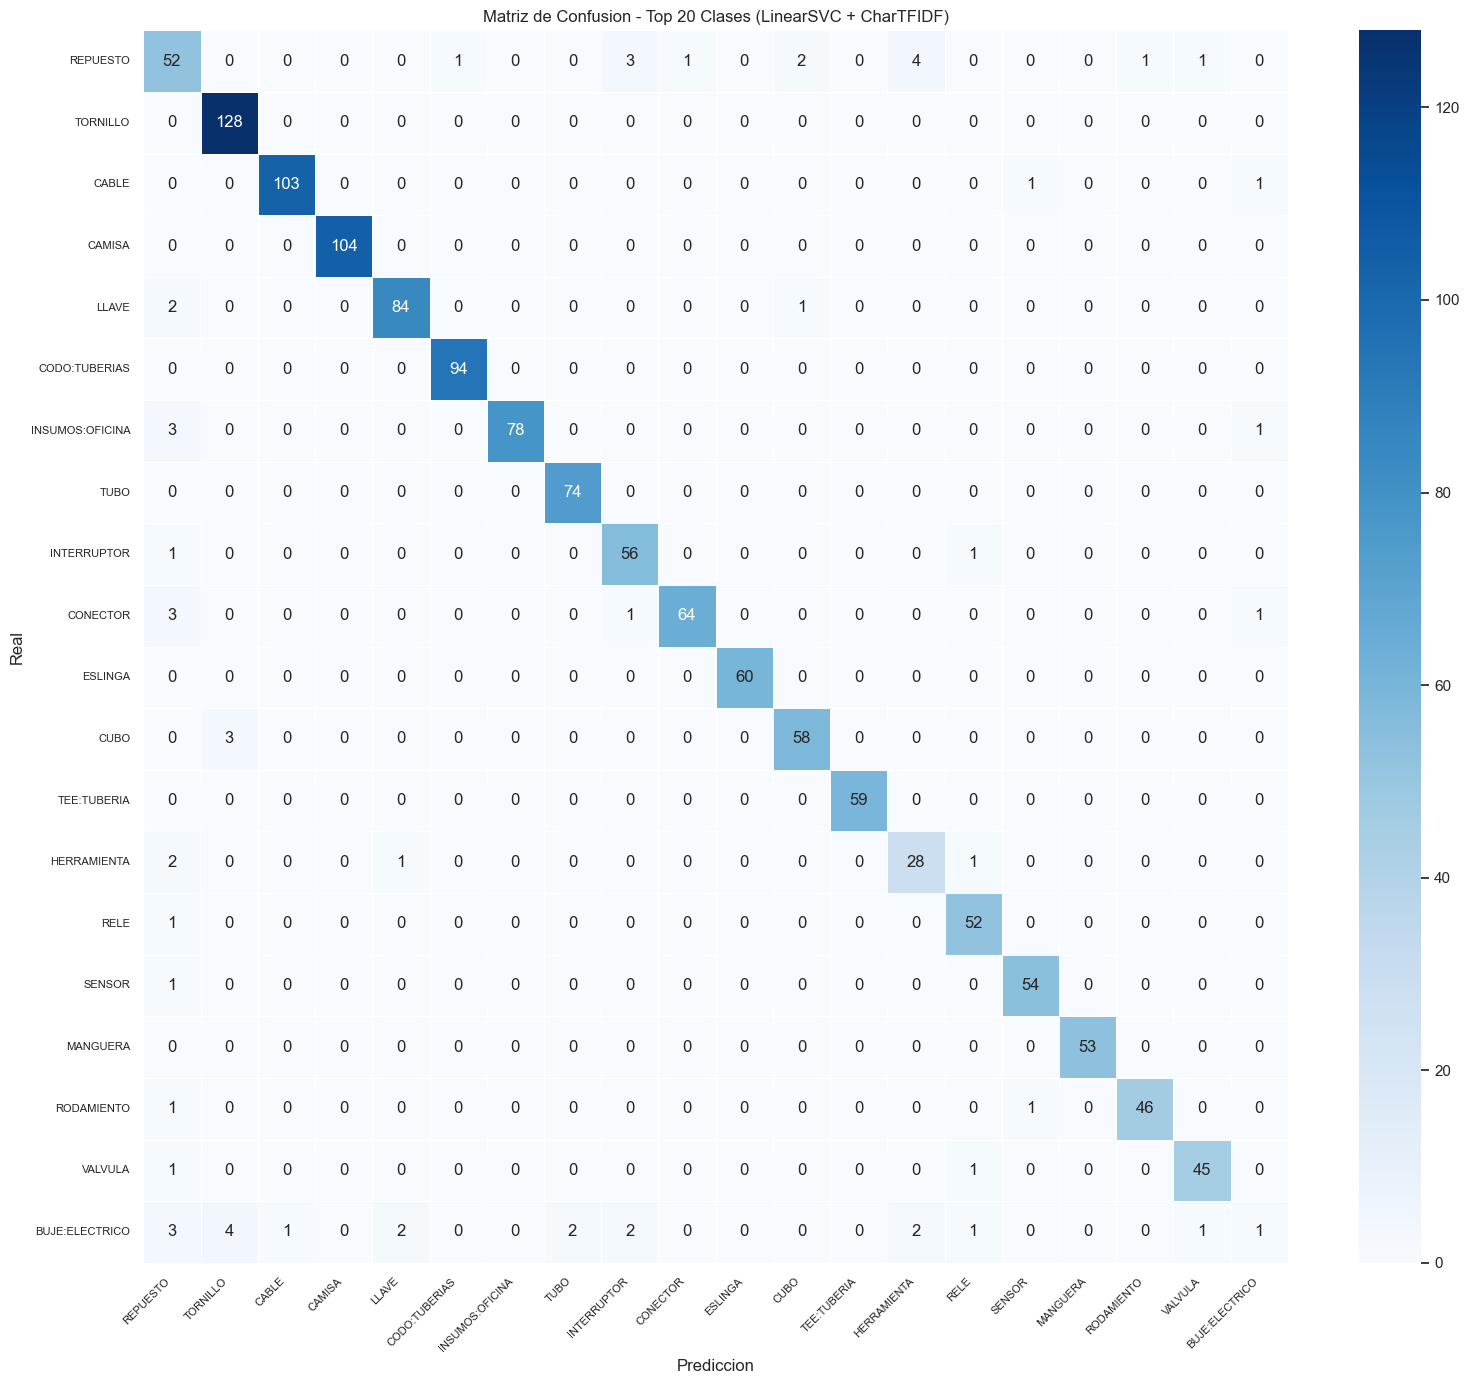
\includegraphics[width=0.92\textwidth]{figuras/modelos/nb02_cell33.png}
\caption{Matriz de confusión del modelo seleccionado sobre las veinte clases de mayor volumen}
\label{fig:matrizconf}
\end{figure}

El modelo cometió 1,194 errores sobre los 7,915 materiales de prueba, equivalentes al 15.09\,\%. El Cuadro \ref{cuadro:confusiones} recoge las diez confusiones más frecuentes.

\begin{table}[!htb]
\centering
\caption{Confusiones más frecuentes del modelo seleccionado sobre la partición de prueba}
\label{cuadro:confusiones}
\small
\begin{tabular}{L{5.4cm}L{5.4cm}r}
\toprule
\textbf{Clase real} & \textbf{Clase predicha} & \textbf{Casos} \\
\midrule
CONTACTOR:ELECT.      & CONTACTO:ELECT.         & 7 \\
TUBO:NO METALICO      & TUBO                    & 6 \\
FUENTE:ALIMENTACIÓN   & FUENTE ALIMENTACION     & 6 \\
CARGADOR DE BATERIAS  & CARGADOR:BATERIAS       & 6 \\
FUSIBLE               & FUSIBLE                 & 5 \\
INTERRUPTOR           & INTERRUPTOR:AUTOMATICO  & 5 \\
REPUESTO              & INTERRUPTOR:AUTOMATICO  & 4 \\
FUENTE ALIMENTACION   & FUENTE:ALIMENTACIÓN     & 4 \\
TRANSFORMADOR         & TRANSFORMADOR:CORRIENTE & 4 \\
BUJE:ELECTRICO        & TORNILLO                & 4 \\
\bottomrule
\end{tabular}
\end{table}

\section{Exactitud y cobertura según el umbral de confianza}
El Cuadro \ref{cuadro:umbral} y la Figura \ref{fig:confianza} presentan el comportamiento del modelo al aplicar distintos umbrales de confianza sobre la partición de prueba.

\begin{table}[!htb]
\centering
\caption{Exactitud y cobertura del modelo seleccionado según el umbral de confianza aplicado}
\label{cuadro:umbral}
\begin{tabular}{crrr}
\toprule
\textbf{Umbral} & \textbf{Exactitud} & \textbf{Cobertura} & \textbf{Materiales cubiertos} \\
\midrule
Sin umbral & 0.8491 & 100.00\,\% & 7,915 \\
0.5        & 0.9280 & 78.81\,\%  & 6,238 \\
0.6        & 0.9484 & 70.50\,\%  & 5,580 \\
0.7        & 0.9674 & 60.52\,\%  & 4,790 \\
0.8        & 0.9862 & 42.25\,\%  & 3,344 \\
\bottomrule
\end{tabular}
\end{table}

\begin{figure}[!htb]
\centering
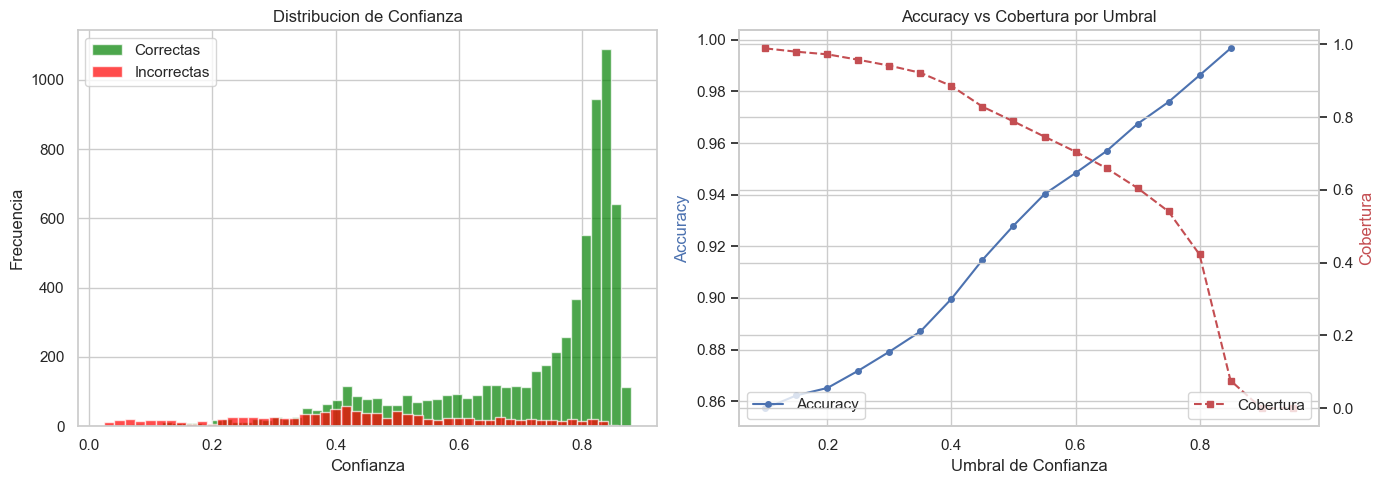
\includegraphics[width=\textwidth]{figuras/modelos/nb02_cell36.png}
\caption{Distribución de la confianza del modelo y compromiso entre exactitud y cobertura según el umbral}
\label{fig:confianza}
\end{figure}

El panel izquierdo de la Figura \ref{fig:confianza} muestra que las predicciones correctas se concentran en la región de confianza alta mientras que las incorrectas se distribuyen hacia valores bajos. Al umbral adoptado por la plataforma, el modelo alcanza una exactitud de 0.9862 sobre el 42.25\,\% de los casos.

\section{Resultados de la operación en producción}

% ============================================================================
% PENDIENTE — resultados del período 18 jun – 21 jul 2026.
% Extraer de las vistas del esquema gold y presentar aquí:
%   · gold.kpi_processing_time  → tiempo de gestión por solicitud
%   · gold.kpi_step_breakdown   → desglose máquina vs. deliberación del gestor
%   · gold.kpi_quality          → exactitud en operación real (tasa de corrección)
%   · gold.kpi_duplicates       → duplicados detectados y evitados
%   · gold.kpi_savings          → ahorro en horas-gestor y en quetzales
%   · gold.kpi_requests_by_user → volumen por gestor
% Verificar antes que gold.parameters tenga los valores reales de
% manual_time_s y hourly_rate (en el repositorio siguen en 0).
% Incluir el número de solicitudes procesadas (n) del período.
% ============================================================================


\chapter{Discusión}

\section{Sobre la selección del algoritmo}
El resultado más relevante de la competencia es que la configuración más simple resultó también la mejor, y por un margen consistente en las cuatro métricas de desempeño. La máquina de vectores de soporte lineal sobre una representación de caracteres superó tanto a los métodos de ensamble como a las arquitecturas basadas en aprendizaje profundo.

La diferencia en costo computacional refuerza esa conclusión. XGBoost consumió más de tres horas de entrenamiento para quedar tres puntos porcentuales por debajo del ganador, que se entrenó en poco más de un minuto; la regresión logística sobre n-gramas de carácter tardó diecisiete veces más que el ganador para un resultado también inferior. En un sistema concebido para reentrenarse periódicamente conforme el catálogo crece, esa diferencia deja de ser un detalle de laboratorio: un modelo que exige horas de cómputo para actualizarse es un modelo que en la práctica no se actualiza.

Este hallazgo es consistente con la naturaleza del problema. Las descripciones del maestro son textos cortos, altamente estructurados y con vocabulario técnico acotado; no contienen la ambigüedad sintáctica ni las dependencias de largo alcance que justifican modelos de mayor capacidad. Un clasificador lineal sobre una representación de caracteres captura precisamente el tipo de regularidad que este texto exhibe.

\section{Sobre el efecto del desbalance de clases}
Todas las configuraciones evaluadas muestran una brecha sistemática entre el F1 macro y el ponderado, de entre nueve y quince puntos según el caso. Esa brecha es la expresión cuantitativa del desbalance descrito en los resultados: los modelos aciertan considerablemente mejor sobre las clases pobladas que sobre las minoritarias, y dado que más de la mitad de las clases cuenta con diez materiales o menos, el promedio no ponderado penaliza con fuerza ese comportamiento.

Resulta significativo que el ordenamiento entre configuraciones no sea idéntico bajo ambas métricas. La regresión logística sobre n-gramas de carácter alcanza la tercera mejor exactitud pero el peor F1 macro del conjunto, lo que indica que su desempeño se concentra desproporcionadamente en las categorías frecuentes. El modelo seleccionado, en cambio, lidera ambas métricas, lo que sugiere un comportamiento más uniforme a lo largo de la taxonomía y no solo un buen resultado agregado.

\section{Sobre el transformador que no convergió}
El resultado obtenido por el transformador multilingüe no corresponde a un modelo que compite y pierde, sino a un entrenamiento que no alcanzó a converger bajo el presupuesto de cómputo disponible. Una exactitud del 3.95\,\% con un F1 macro prácticamente nulo indica que el modelo no llegó a diferenciar las categorías, no que la arquitectura sea inadecuada para la tarea.

La explicación más probable combina la dimensionalidad del problema —1,234 clases de salida— con un número de épocas y una configuración de ajuste fino insuficientes para adaptar un modelo preentrenado en lenguaje general a un vocabulario técnico especializado, requerimiento que la literatura documenta como característico de esta familia \cite{vaswani2017}. La cifra se reporta por transparencia del procedimiento, pero no admite lectura como evidencia sobre el desempeño potencial de los transformadores en esta tarea. Su evaluación adecuada requeriría un presupuesto de cómputo que excedía el alcance del proyecto, y queda planteada como línea de trabajo posterior.

\section{Sobre la naturaleza de los errores del modelo}
El examen de las confusiones más frecuentes arroja el hallazgo de mayor alcance del análisis, y trasciende el desempeño del modelo. La mayoría de esos casos no son errores de clasificación en sentido estricto, sino manifestaciones de un problema del propio catálogo: existen pares de clases que designan el mismo concepto y difieren únicamente en puntuación, acentuación o separador.

Los pares \textit{FUENTE:ALIMENTACIÓN} y \textit{FUENTE ALIMENTACION}, o \textit{CARGADOR DE BATERIAS} y \textit{CARGADOR:BATERIAS}, son clases distintas en la taxonomía pero indistinguibles en su significado. El caso más elocuente es el de \textit{FUSIBLE} confundido consigo mismo, que solo puede corresponder a dos códigos de clase homónimos coexistiendo en el catálogo. Ninguna representación del texto puede discriminar entre categorías que son semánticamente idénticas: una fracción del error medido es irreducible mientras la taxonomía no se depure.

Esto tiene dos implicaciones. La primera es metodológica: la exactitud del 84.91\,\% subestima el desempeño real del modelo, ya que una parte de sus errores consiste en asignar una etiqueta correcta que la taxonomía duplica bajo otro código. La segunda es operativa: el análisis de errores del modelo constituye, por sí mismo, un instrumento de diagnóstico de la calidad del catálogo, capaz de señalar los pares de clases candidatos a fusión. La herramienta construida para clasificar materiales resultó también un mecanismo para detectar defectos en la taxonomía que los clasifica.

Las categorías genéricas constituyen el segundo foco de error. Clases como \textit{repuesto} o \textit{herramienta} no designan un objeto sino una función, y por lo tanto carecen de vocabulario distintivo: un repuesto puede ser cualquier cosa. Su baja tasa de acierto no refleja una deficiencia del modelo sino una debilidad de diseño de la taxonomía, que admite categorías sin contenido descriptivo.

\section{Sobre el punto de operación seleccionado}
La caracterización del compromiso entre exactitud y cobertura permite fundamentar con datos una decisión que de otro modo sería arbitraria. Al umbral adoptado, el sistema acierta en el 98.62\,\% de los casos que resuelve de forma automática, a cambio de derivar a revisión del gestor algo más de la mitad de las solicitudes.

Se privilegió deliberadamente la exactitud sobre la cobertura, y la justificación es de costos asimétricos: en un proceso de gobierno de datos, una categoría incorrecta que ingresa al catálogo sin revisión genera un costo persistente —distorsiona reportes de consumo, complica la planificación de compras y se propaga a todo proceso que consulte el catálogo—, mientras que una sugerencia derivada a revisión solo consume la atención del gestor, que es exactamente el escenario que la herramienta está diseñada para atender. Conviene subrayar que incluso las solicitudes derivadas a revisión conservan valor: el gestor recibe tres candidatos ordenados por probabilidad en lugar de enfrentar el catálogo completo.

La forma de la distribución de confianza respalda la validez del procedimiento. Que las predicciones correctas se concentren en la región de confianza alta y las incorrectas se dispersen hacia valores bajos es la condición que hace útil cualquier umbral; si la confianza no discriminara entre aciertos y errores, la predicción selectiva carecería de sentido.

\section{Comparación con los antecedentes}
El desempeño obtenido admite una lectura comparativa frente al antecedente más cercano identificado en la literatura. \citeA{ding2002}, clasificando descripciones de producto contra la taxonomía UNSPSC, reportaron una exactitud del 78\,\% en la primera predicción y del 88\,\% sobre las diez primeras sugerencias, discriminando entre 421 categorías.

El modelo desarrollado en este proyecto alcanza 84.91\,\% y 94.04\,\% respectivamente, sobre 1,234 categorías y con una ventana de sugerencias considerablemente más estrecha, ya que su segunda cifra se mide sobre tres opciones y no sobre diez. Debe insistirse en que ambos resultados provienen de conjuntos de datos distintos y no constituyen una comparación controlada; su valor es el de situar el desempeño obtenido dentro del orden de magnitud que la literatura reporta para esta clase de problema.

En ese marco resulta especialmente pertinente la advertencia de esos mismos autores: una exactitud en el rango del 78 al 88 por ciento iguala o supera la calidad de la clasificación humana sobre el mismo material, y perseguir cifras sensiblemente superiores implicaría sobreajustar el modelo a decisiones humanas que a su vez contienen una tasa de error no despreciable. La observación aplica de manera directa a este proyecto, cuyo conjunto de entrenamiento son precisamente las clasificaciones históricas realizadas por los gestores, con los defectos de taxonomía que el análisis de errores puso de manifiesto.

\section{Limitaciones del estudio}
Los resultados presentados deben interpretarse dentro de varias limitaciones.

La primera concierne a la evaluación del modelo. La convención de nomenclatura del catálogo hace que el término principal de la descripción coincida con frecuencia con el nombre de la clase a la que el material pertenece, de modo que una parte del desempeño observado es atribuible a esa correspondencia léxica directa. Cuantificar qué proporción del acierto depende de ella requeriría una evaluación por ablación, eliminando el término inicial de la descripción y midiendo la caída resultante. Ese ejercicio no se realizó y queda planteado como verificación pendiente.

La segunda es que el modelo se entrena sobre etiquetas producidas por los propios gestores, que constituyen la mejor referencia disponible pero no una verdad de campo independiente. El techo de desempeño alcanzable está determinado por la consistencia de esas decisiones históricas.

La tercera se refiere al alcance de la validación. El período de uso productivo abarca cinco semanas y una sola unidad de negocio, frente a una línea base levantada durante cuatro meses. La asimetría entre ambos períodos y el tamaño de la muestra acumulada aconsejan tratar las cifras de la operación como indicativas de una tendencia y no como estimaciones de precisión estadística.

Finalmente, los resultados de clasificación se obtuvieron sobre una fotografía del catálogo correspondiente a una fecha determinada. El desempeño del modelo sobre materiales de familias que no estaban representadas en esa extracción no puede inferirse de las mediciones presentadas.
